%% It is just an empty TeX file.
%% Write your code here.
\chapter{Communication System Test}\label{ch:experiment}

\section{Functional Shorts Implementation}
To verify the functional test concept an example communication system has been built and shown in \autoref{fig:short_ena}. The implementation lacks real modules, except from the encoder and decoder. Every other module is implemented as a simple delay in the digital information flow (flip flop) and XOR gate to conduct the error injection. They also have special enable signal to choose which module should occur as faulty. The AIR simulates the communication channel. There is also a programmable delay to variate the execution time of the test and to simulate the fact that the number of clock cycles, needed for the information to pass from the encoder to decoder, is not constant in all tests. The short enable signals control the data flow in the test loop. The activation of any short, excludes the whole part of the system laying beyond the short and shortens the test duration, because the information doesn't need to be clocked through all excluded modules. The injected error vector travels through the design together with the test data. This guaranties the proper alignment of the error vector with the test vector at any time, also during the shortcut, when the path is shorter. The error vector flips the specified bits of the output of any chosen module to simulate the possible effects of hardware faults on the processed information. The error enable signal is exclusive, meaning that only one module may be faulty at the same time. 

\begin{figure}[h]
\centering
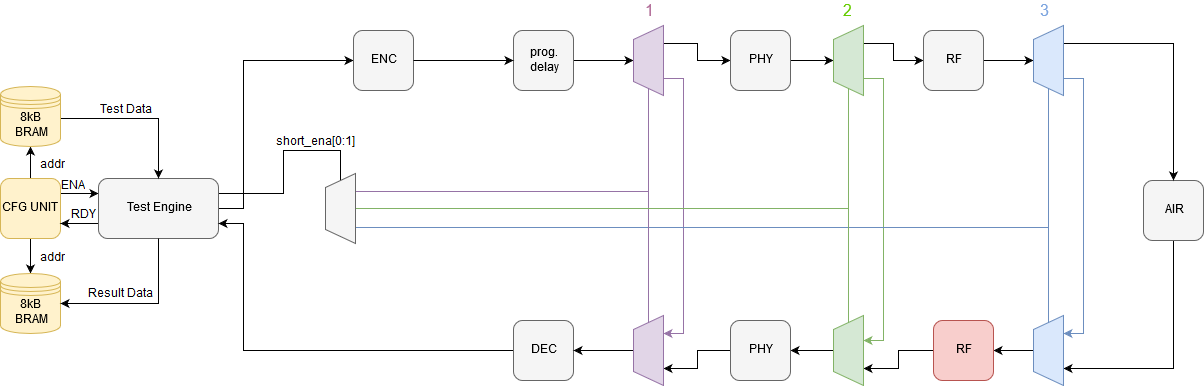
\includegraphics[width=\textwidth]{figures/Short_ena_err.png}
\caption{Implementation of functional shorts into the Test Bench}
\label{fig:short_ena}
\end{figure}

The experimental set-up has been implemented into the Test Bench. It consists of the BCH(1023,943) Encoder and Decoder, being able to correct up to 8 bit errors. The encoder and decoder need a reset signal to start working. The reset is followed by 943 random data bits and 80 zeros to compute the parity bits in the encoder. Parallel to these 1023 encoder bits, a 1023 bit error vector is shifted in. The bit that is supposed to be flipped is set to one, the rest to zero. The data block and the error vector are appended by the zero vector of the following length. The size of the programmable delay plus one for every module in the current test loop. The excluded modules laying beyond the active short, are not counted. The decoder needs additional 97 clock cycles for syndrome calculations and error localization, therefore another 97 zeros need to be added to the input signals. To shift out the corrected user bits another 943 cycles are needed. To monitor the error detection in the whole block, another 80 bits can be shifted out. The decoder response lies in the last 1023 bits of the output bitstream, so do 1023 special output bits, indicating the correction.

To detect that the RF part of the receiver is faulty, following steps need to be taken:
\begin{enumerate}
    \item Start the test by enabling the shortcut nr. 3, closing the test loop between transmitter and receiver
    \item Conclude the test by running all test vectors through the design, placing them on the inputs of FEC encoder, until the first occurrence of the ISERR set high
    \item Enable shortcut nr. 2
    \item Run test again and detect no errors, since the faulty unit is not in the test loop
    \item Run repair procedure on the transmitter RF unit
    \item Enable Shortcut nr. 2
    \item Run the test only to see the ISERR is high again
    \item Run repair procedure on RF unit of the receiver, revert the repair of the transmitter RF unit
    \item Start the test again to see no errors detected
\end{enumerate}

All tests revealed that the method can be used for systematic fault diagnosis on the module level. Systematic exclusion of modules and test repetition allowed to localize a faulty module in all cases. The number of errors was lower or equal to the correction capability of the decoder. But how do the system react to the higher number of errors and what real errors occur as result of real permanent faults? Firstly the BCH encoder was tested for errors resulting from delay faults. Then fault injection was conducted to observe how the encoder reacts in presence of transient and permanent faults. Then the decoder was tested for error detection above its maximal correction capability and also for delay faults.

\section{Test of BCH(1023,943) Encoder}
The tested encoder is a BCH encoder taking 943 payload bits and calculating 80 parity bits. The encoder is actually a part of the PENCA architecture, without any redundant test and configuration circuitry. The encoder consists of an LFSR for parity calculations and the counter to keep track on the number of input user bits. Before the counter reaches 943 bits, it forwards the user bits to the output and enables linear feedback in the shift register. Then the parities are shifted out with "dummy" input bits with the LFSR acting as simple shift register. The parity calculation is obtained by dividing the input polynomial by the generator polynomial of the encoder. The reminder of the division is the parity polynomial. The general architecture of a BCH encoder using a LFSR for polynomial division is shown in \autoref{fig:enc_0}. Since the test bench developed during the project allows a test with wide range of frequencies, it may be possible to cause some delay faults in the encoder architecture and examine, how they influence the output bit stream.

\begin{figure}[h]
\centering
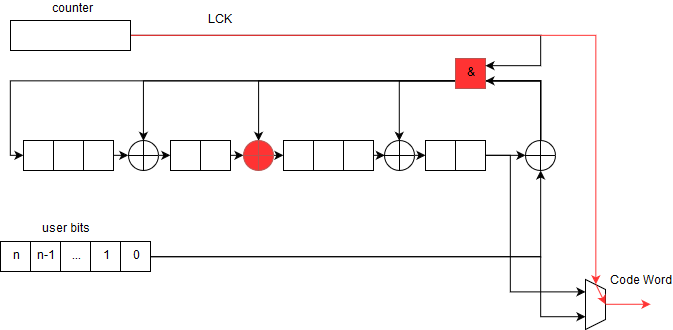
\includegraphics[width=0.65\textwidth]{figures/BCH_ENC.png}
\caption{A BCH encoder architecture \cite{art:BCH_implement}}
\label{fig:enc_0}
\end{figure}

The encoder has been placed in the test bench and tested for maximum frequency. The input data is random. There were 300 messages sent and evaluated. The comparison data was calculated using MATLAB 2015b comm.BCHEncoder. There were two encoder versions tested. One version is surrounded by flip-flops to guarantee that the delay fault happens in the encoder design and not due to the long connection paths between encoder design and the Test Engine. This version was called "isolated". The "not isolated" one was connected simply to the input and output registers of the Test Engine. First clock cycle is reserved for the reset. When the reset is low, the input vector is shifted in serially. The output is equal to the input when the payload bits are shifted in. After 943 payload bits, the input is set to zero and held that way till the end of the test, which means another 80 clock cycles for the parity bits to be shifted out. The test fails when the output value is different from the pre-calcualted value. The frequency is raised until first tests start to fail. This marks the cut-off frequency of the Encoder and reveals the errors caused by delay fault. The cut-off frequencies are presented in \autoref{tab:enc}.

\begin{table}[h]
\begin{tabular}{@{}lllll@{}}
\toprule
UUT                       &mem\_width   &uut\_width &expected freq. &max. freq.\\ 
\midrule
isolated Encoder                  & 32          & 4      & $\sim$642 MHz & $\sim$500 MHz \\
not isolated Encoder              & 32          & 4      & $\sim$642 MHz & $\sim$326 MHz \\
\bottomrule
\end{tabular}
\centering
\caption{Test Encoder for max. frequency}\label{tab:enc}
\end{table}

The result shows clearly that a Test Engine limit of 500 MHz has been reached while testing the isolated Encoder, the frequency was not raised above this value, because the result would not be reliable. The not-isolated version on the other hand, failed by the frequency of 326 MHz. Both versions differ only in flip-flops isolating them from the test bench, therefore any errors happening in the not-isolated version did not arise in the Encoder itself. They originate from the long connections between the Encoder and the Test Bench. But such errors could also arise due to delay faults in real hardware. 

\autoref{fig:enc_1} represents the result of all failed test of the not-isolated Encoder at approx. 355 MHz. In half of the messages the first parity bit is corrupted. When the counter, calculating the number of shifted bits, reaches the 943, the output should be switched to the parity bits (see \autoref{fig:enc_0}). In all vectors, the output still forwards the input value, which is zero for all "dummy" parity bits. In half of the vectors, since they are randomly distributed, the zero is accidentally the expected value, therefore the error gets masked.

The raised frequency together with very long interconnect simulated a delay fault in the control signal of the multiplexer. It is marked as red line in \autoref{fig:enc_0}. When the counter reaches 943, a special LCK signal is generated to disable feedback in the LFSR and change the source of the output pin to forward LFSR output instead of Encoders input. The outcome is a single bit error in half of the produced code words. This error can be easily detected and corrected by the decoder.

\begin{figure}[h]
\centering
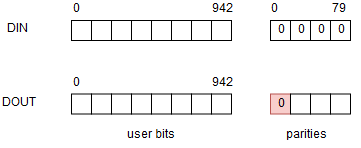
\includegraphics[width=.5\textwidth]{figures/enc_error.png}
\caption{The result of failed Encoder test by 355 MHz}
\label{fig:enc_1}
\end{figure}

Designing with FPGAs, allows to build in some additional functions into existing IPs. To examine the influence of real hardware faults, a special fault injection was built into the encoder design. The output of the gates, marked red in \autoref{fig:enc_0}, has been manipulated in a way showed in \autoref{fig:error_injection}. The manipulated gate in the LFSR resides between the 52nd and 53rd register. Since the Test Engine is a synchronous design, there is no possibility to simulate single event transients lasting less than a single clock cycle, without manipulating the design even further. The values on inputs are constant throughout the whole clock cycle, so only SEU injection is possible. The inputs are called $SA1$ and $SA0$, after the logical levels at the output of error injecting logic, after the error injection. The $SA0$ takes precedence, because the AND gate is positioned last. The error injection logic allows to produce permanent faults (stuck-at faults), when one of the inputs is held high throughout the whole test, or transient faults (SEU) when one of the inputs is set high occasionally.

\begin{figure}[h]
\centering
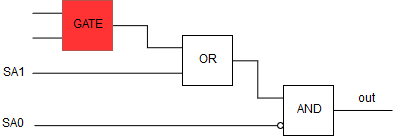
\includegraphics[width=.5\textwidth]{figures/error_injection.png}
\caption{The result of failed Encoder test by 355 MHz}
\label{fig:error_injection}
\end{figure}

The effects of permanent faults in the feedback, both SA0 and SA1, were destructive and resulted in all parities stuck at 0, as if the encoder did not exist in the circuit. It made the generator polynomial have no influence on the rest of LFSR. The permanent faults in the shift register also influenced all parity bits, but in a different way. The last 54 parities were stuck at the value injected, the rest was randomly flipped. No permanent error was masked, since all data need to pass trough afflicted gates.

The effects of transient faults were observed by injecting only SA1 faults in both places. In both places only one SEU was caused, by holding the appropriate input high for one clock cycle. This time only 50\% of all blocks failed, since the injected error does not flip a bit, but sets it to 1 or 0. The injected value was expected in half of the messages. Even a single SEU caused multiple error bits in most cases. The only exceptions were errors caused by faults happening during the shift operation, when the linear feedback was disabled. A fault injected in the shift register caused a single bit error, because it only influenced one register and the erroneous value was simple shifted out. A fault in feedback caused multiple bit error, because it enabled the feedback for one clock cycle and influenced all bits connected to it, still residing in the shift register. The later the fault happened, the less bits were afflicted. Fault effects are much smaller when the linear feedback is disabled.


\section{Test of BCH(1023,943) Decoder}

For any positive integers $m \geq 3$ and $t<2^{m-1}$ there exists a binary BCH code with the following parameters \cite{art:BCH_implement}:
\begin{subequations}
\begin{align}
    \text{block length }n&=2^{m}-1\label{eq:blck_len}\\
    \text{parity bits }k&\geq n+mt\label{eq:parity}\\
    \text{hamming distance }d&\geq2t+1\label{eq:dmin}
\end{align}
\end{subequations}
The BCH(1023,943) with its $n = 1023$ and $k=943$, has a $d_{min}= 17$. The code is therefore capable of detecting 16 error bits and correcting 8 in a single block. 

The tested BCH decoder has one serial data input (DIN) and one data output (DOUT). The input data enters the syndrome computation block, which is similarly to encoder, implemented as a LFSRs. It is actually less complicated than the encoder, having shorter LFSRs to compute partial syndromes, one for every correctable error. When all syndromes are equal zero, the received message is a valid code word. In other case, when any syndrome is non-zero, the Key Equation Solver has to find the parameters of error locating polynomial. The parameters are passed to Chien Search Block to find the roots of the error locating polynomial and therefore the exact positions of errors in the received message. The output of the Chien Search Block is connected to the output ISERR to indicate, if the current output bit has been repaired. This is the special extension allowing the Functional Short Concept to be implemented. The decoder needs 97 clock cycles before it starts shifting out the corrected user bits. The basic idea of building a BCH Decoder is shown in \autoref{fig:dec_0}.

\begin{figure}[h]
\centering
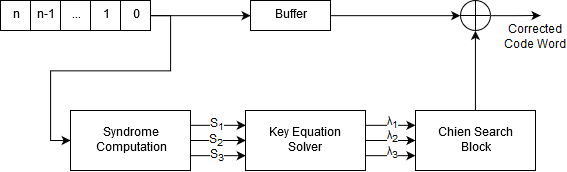
\includegraphics[width=0.65\textwidth]{figures/BCH_DEC.png}
\caption{A BCH decoder architecture \cite{art:BCH_implement}}
\label{fig:dec_0}
\end{figure}

\subsection{Test Decoder for maximal frequency}

The test procedure involving functional shortcuts assumed a fault free functionality of the decoder. It is possible though that the decoder suffers from any permanent or transient fault itself, giving false negative or false positive results of the test, not mentioning the problems during normal communication. The knowledge about possible errors is important. The following tests try to cause some delay faults in the decoders architecture.

The decoder was tested for its maximal operational frequency and beyond. The decoder was tested only until its maximal correction capabilities, meaning 8 injected errors. The error injection happens statically during the data generation. The data is generated in steps. Firstly, 943 random bits are processed by the comm.BCHEncoder block in MATLAB. Then, the coded bitstream is XORed with an error vector with random error positions, but constant hamming weight, creating a data input for the decoder test. The expected result is the output of the MATLAB block, before error injection. The hamming weight of the error vector was increased from 1 to 8 and tested for maximum frequency. The results are summarized in \autoref{tab:dec}
\begin{table}[h]
\begin{tabular}{@{}ccccll@{}}
\toprule
UUT                       &mem\_width   &uut\_width &error cnt. &\begin{tabular}{@{}c@{}}unconstrained \\max. freq.\end{tabular} &\begin{tabular}{@{}c@{}}constrained \\max. freq.\end{tabular}\\ 
\midrule
\multirow{9}{*}{\begin{tabular}{@{}c@{}}isolated \\Decoder\end{tabular}}    & \multirow{9}{*}{32}        & \multirow{9}{*}{8}       &0           & $\sim$264 MHz & $\sim$319 MHz \\
                            &                           &                           &1          &   $\sim$237 MHz &   $\sim$229 MHz\\
                            &                           &                           &2          &   $\sim$200 MHz &   $\sim$221 MHz\\
                            &                           &                           &3          &   $\sim$200 MHz &   $\sim$219 MHz\\
                            &                           &                           &4          &   $\sim$200 MHz &   $\sim$219 MHz\\
                            &                           &                           &5          &   $\sim$180 MHz &   $\sim$218 MHz\\          
                            &                           &                           &6          &   $\sim$160 MHz &   $\sim$219 MHz\\
                            &                           &                           &7          &   $\sim$160 MHz &   $\sim$218 MHz\\
                            &                           &                           &8          &   $\sim$160 MHz &   $\sim$219 MHz\\
\bottomrule
\end{tabular}
\centering
\caption{Test Decoder for max. frequency}\label{tab:dec}
\end{table}

The isolated version means that the design was surrounded by flip-flops and the unconstrained design allows the tool to automatically place the design in the FPGA. The direct input and output are always compared with their delayed pairs to check, if the delay fault did not happen on the interface with the Test Bench. The isolation itself did not prevent delay faults on interconnects to manifest and influence the test results. When the frequency was raised above 300 MHz, the unconstrained decoder started to have errors on $DOUT$ output without errors on $ISERR$ output. This situtation is not possible, since the $ISERR$ signal is responsible for flipping the $DOUT$ bits. Hence the error happens in the decoders interface although the design was isolated with additional flip-flops. Both, the delayed and direct paths were erroneous, which prevented those faults from being detected. The reason was the design placement. In the unconstrained version, the placing tool decided to place the isolating registers far away from the decoder and close to the Test Engine. This made the isolation useless and didn't allow to detect the delay faults happening on the interconnects with the Test Engine. Constraining the design was the only way to force the tool to make the isolating registers part of the decoder design and in consequence, to detect interconnect faults. The unconstrained design is presented in \autoref{subfig:uncon}, while the constrained design is showed in \autoref{subfig:con}.

\begin{figure}[h]
\centering
\begin{subfigure}{.45\textwidth}
    \centering
    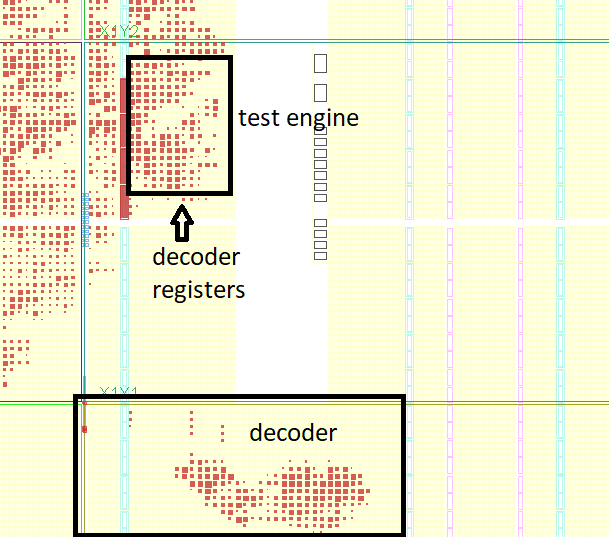
\includegraphics[width=\linewidth]{figures/Device_edited.png}
    \caption{Unconstrained}
    \label{subfig:uncon}
\end{subfigure}%
\hspace{\fill}
\begin{subfigure}{.45\textwidth}
    \centering
    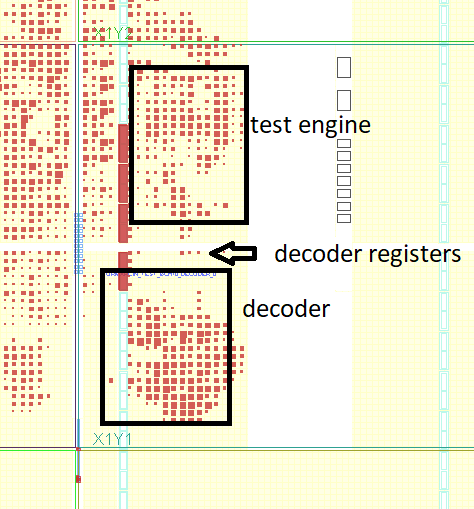
\includegraphics[width=\linewidth]{figures/Device_Pblock_edited.png}
    \caption{Constrained}
    \label{subfig:con}
\end{subfigure}
\caption{Decoder placement in FPGA}
\label{fig:dec_routing}
\end{figure}

The Pblocks are areas in the FPGA that force the placement tool to try to fit parts of the design inside of them. After drawing the Pblock between the old decoder position and the test engine, the decoder was placed closer to the test engine, so the delay fault at the interconnect should appear later and the delayed and direct signal should differ. The detection of delay faults at interconnects is now possible. The tests of constrained design showed that the maximal frequencies were higher, because the distances between various cells were smaller. The design has been closed in smaller space, making the circuit more dense and the cells were repositioned. The maximal frequencies of the constrained design have been presented in \autoref{tab:dec}.

The XML file returned by the test engine allows to examine the failed tests and see where the errors occur and in what number. Every test at cut-off frequency simulates some delay faults and shows the misbehavior of the longest paths in the design. The first test was conducted on isolated constrained design of the decoder. There were 1000 code words sent and every code word had one injected error. At normal frequency, this amount of errors is easily correctable by the decoder, but at the cut-off frequency, the decoder starts to produce some errors by itself. The cut-off frequency for the decoder with 1 injected error is 229 MHz. The test was conducted with 230 MHz. The result of the test is summarized in 3 subfigures in \autoref{fig:dec_3}. 


\begin{figure}[h]
\centering
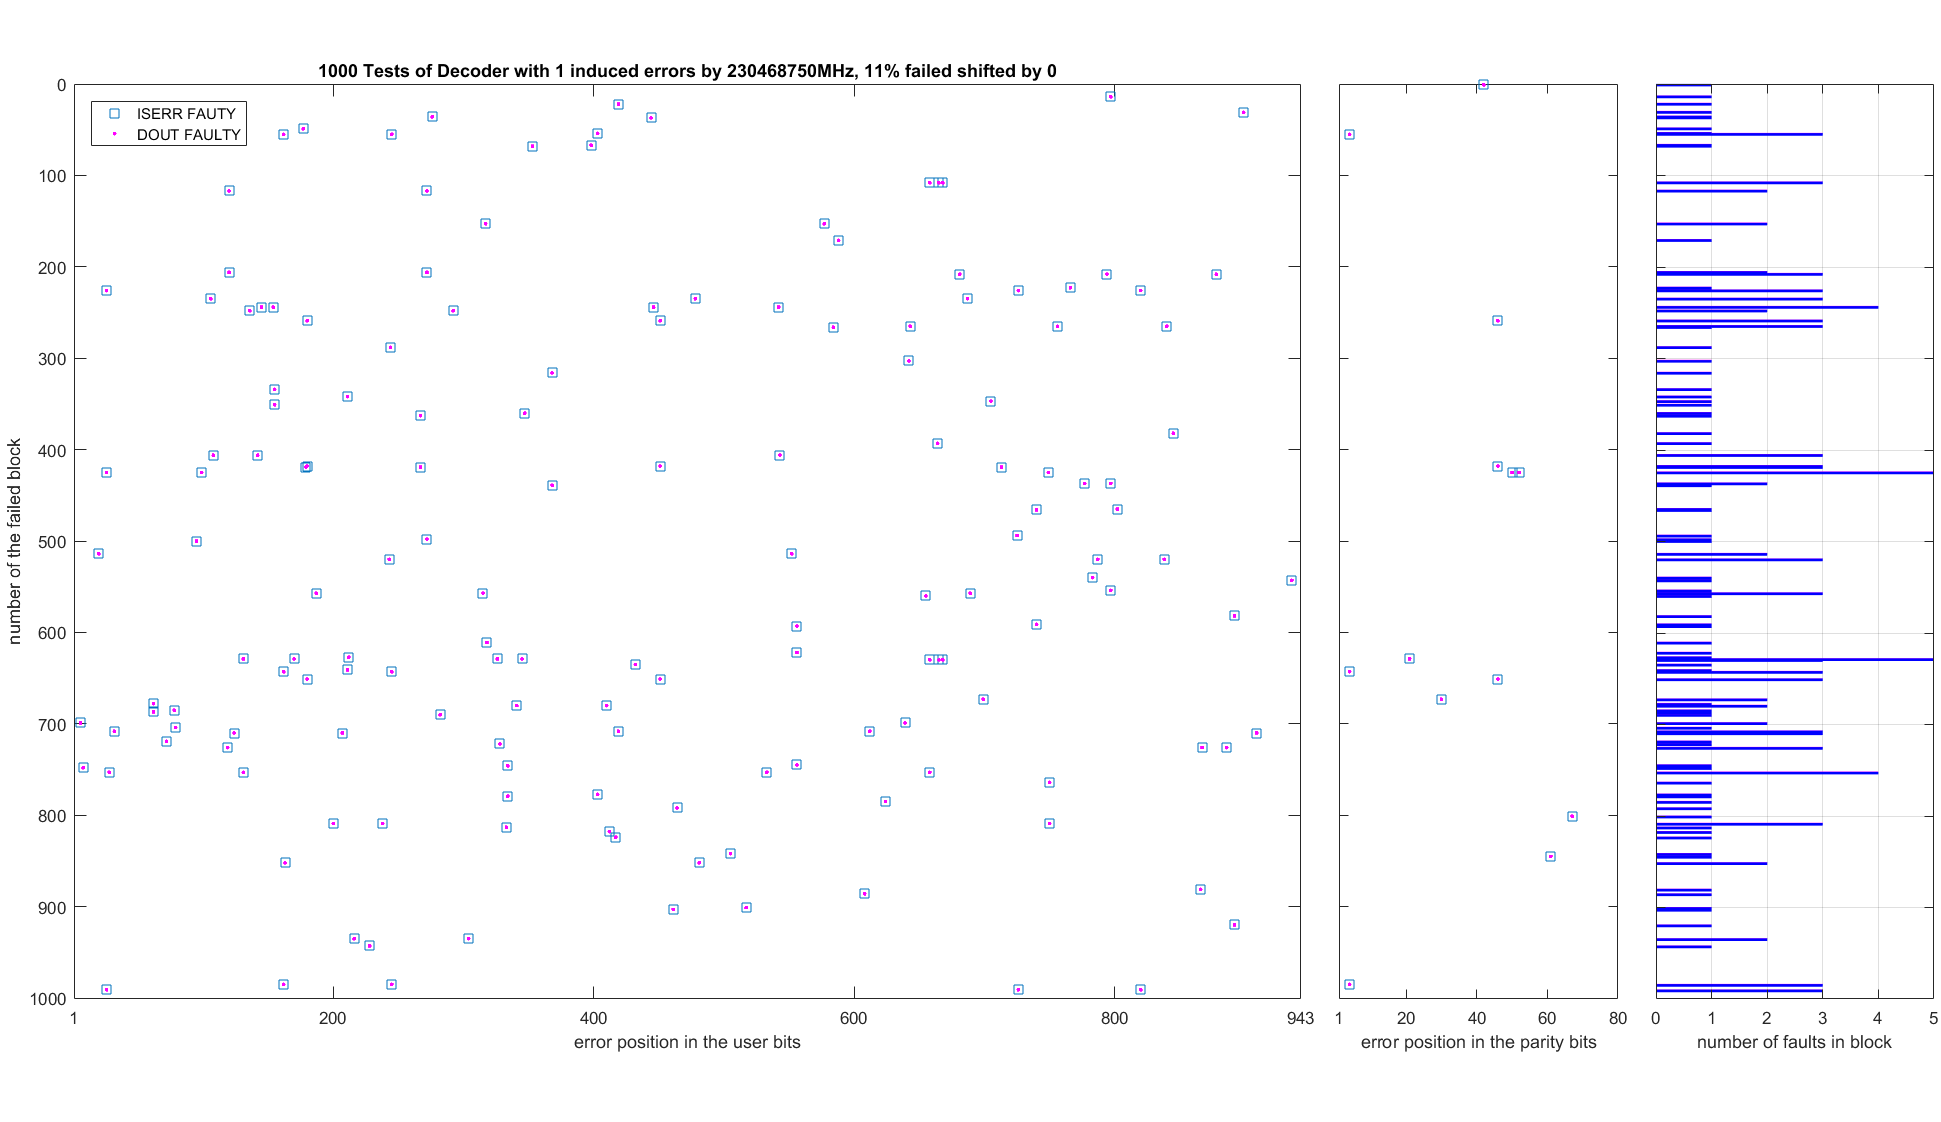
\includegraphics[width=\textwidth]{figures/1000_tests_decoder_overtacted_230_1_error.png}
\caption{Test of BCH Decoder with 1 injected error over the cut-off frequency}
\label{fig:dec_3}
\end{figure}

The most left hand-side subfigure represents the user bits of the received code word, containing 1000 received code word, each 943 bits long. The middle figure represents the received parity bits 1000 code words with 80 parities. Every rectangle with a dot represents an error that the decoder produced by itself. The expected results were calculated using the MATLAB 2015b comm.BCHDecoder.

The error distribution is random, data dependent. For the decoder to produce an error, either the syndrome calculation failed or the Key Equation Solver or Chien Search Block. The single syndrome computation is very similar to the parity computation in the encoder, since it also involves LFSR. The encoder test revealed that a LFSR doesn't fail at such low frequency, hence the errors are produced somewhere in the Key Solver or Chien Search Block. If the Chien Search Block failed, it could produce more errors, than the theoretical decoder correction capability. Such thing was not visible during any of the tests. The fault is therefore probably in the Key Equation Solver or in the control logic.

Another interesting problem is the behavior of the decoder when no errors are injected. During the cut-off frequency test, the maximal frequency for isolated constrained decoder was 319 MHz. After sending 1000 valid code words, with no errors injected and raising the test frequency to 320 MHz, the decoder started to produce rather repeatable errors. The result is showed in \autoref{fig:dec_2}.

\begin{figure}[h]
\centering
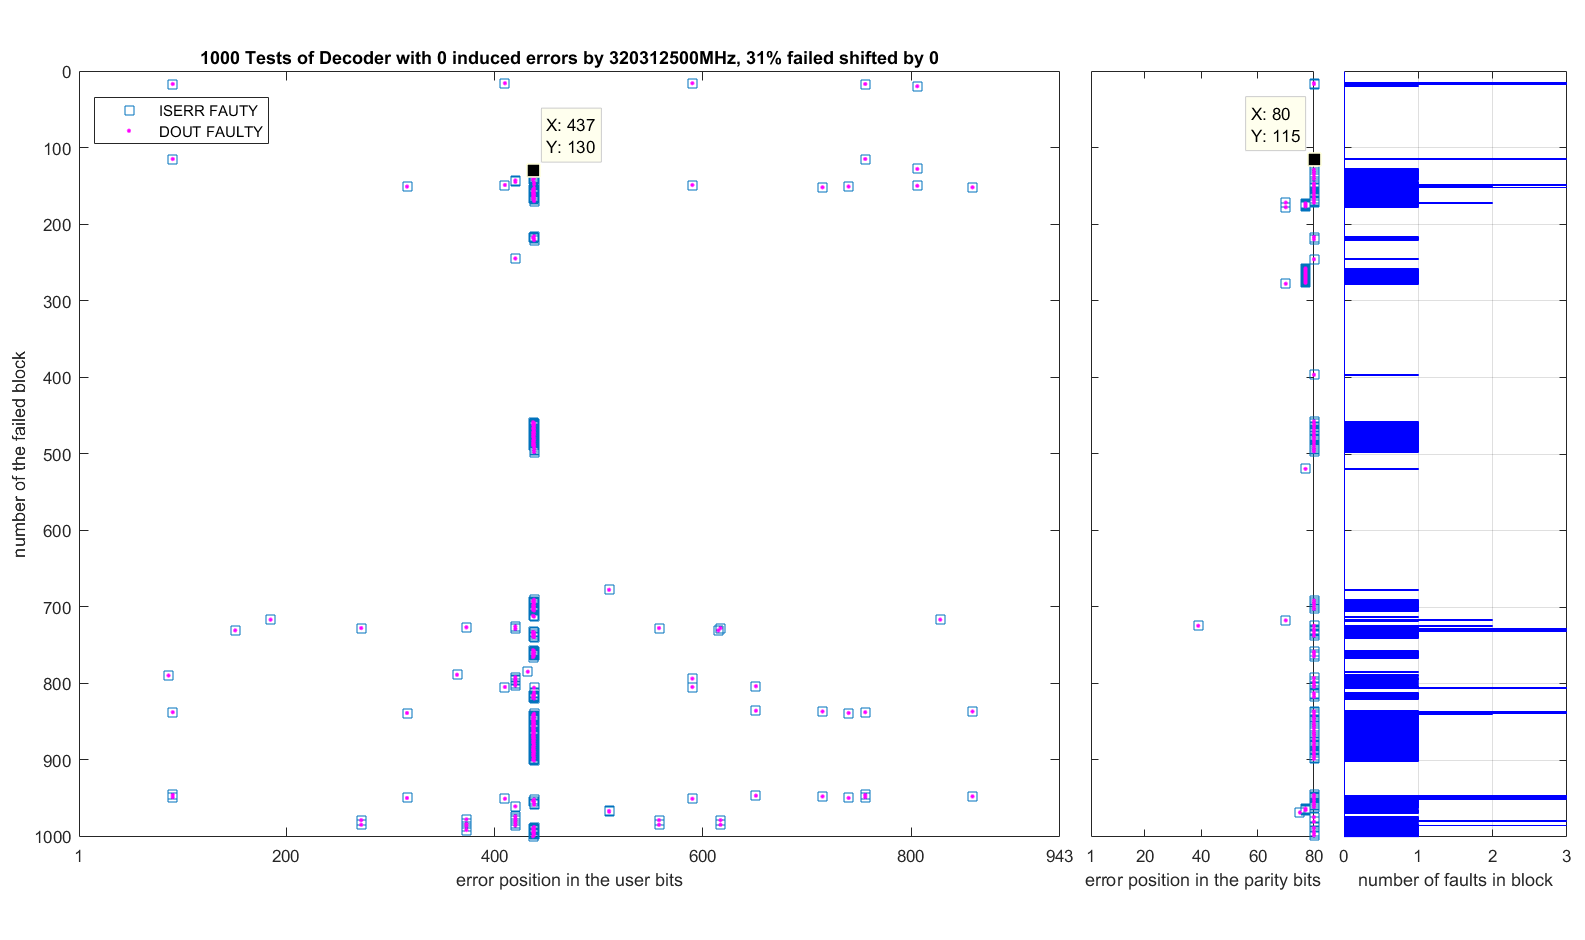
\includegraphics[width=\textwidth]{figures/Test_DDEC_0_fault_1000_320_MHz.png}
\caption{Test of BCH Decoder with 0 injected errors over the cut-off frequency}
\label{fig:dec_2}
\end{figure}

In the test with no injected errors, the syndromes and therefore the parameters of error location polynomial should be zero at all times. The syndromes calculated with use of LFSR should be correct at this frequency. Again the Key Equation Solver is probably responsible for this error patterns.


\subsection{Test Decoder for Maximal Error Detection and Correction}

In the Functional Short Test, only the ISERR output is monitored, since the data is irrelevant. In normal function, the decoder returns only 943 corrected user bits. Upon detection of an error in the parity bits only, no correction is necessary, since the user bits are not changed. In the tested decoder however, the information about erroneous parity bits is easily accessible by monitoring the $ISERR$ output for another 80 clock cycles. The observation of 80 check bits is crucial in error detection, since the whole vector travels through the tested design and can be disturbed in any position, not only in the user bit space. Loosing the information about the 80 check bits, would make some errors undetectable, like all errors happening inside of an encoder, which happen only to the parity bits. 

The underlaying BCH code is capable of correcting 8 bit errors and detecting 16. \autoref{fig:dec_1} shows a result of a simple test, where randomly generated data was "XORed" with randomly generated error vectors with raising hamming weight. Each test consists of 1000 messages and the error number is raised from 1 to 18. 

\begin{figure}[h]
\centering
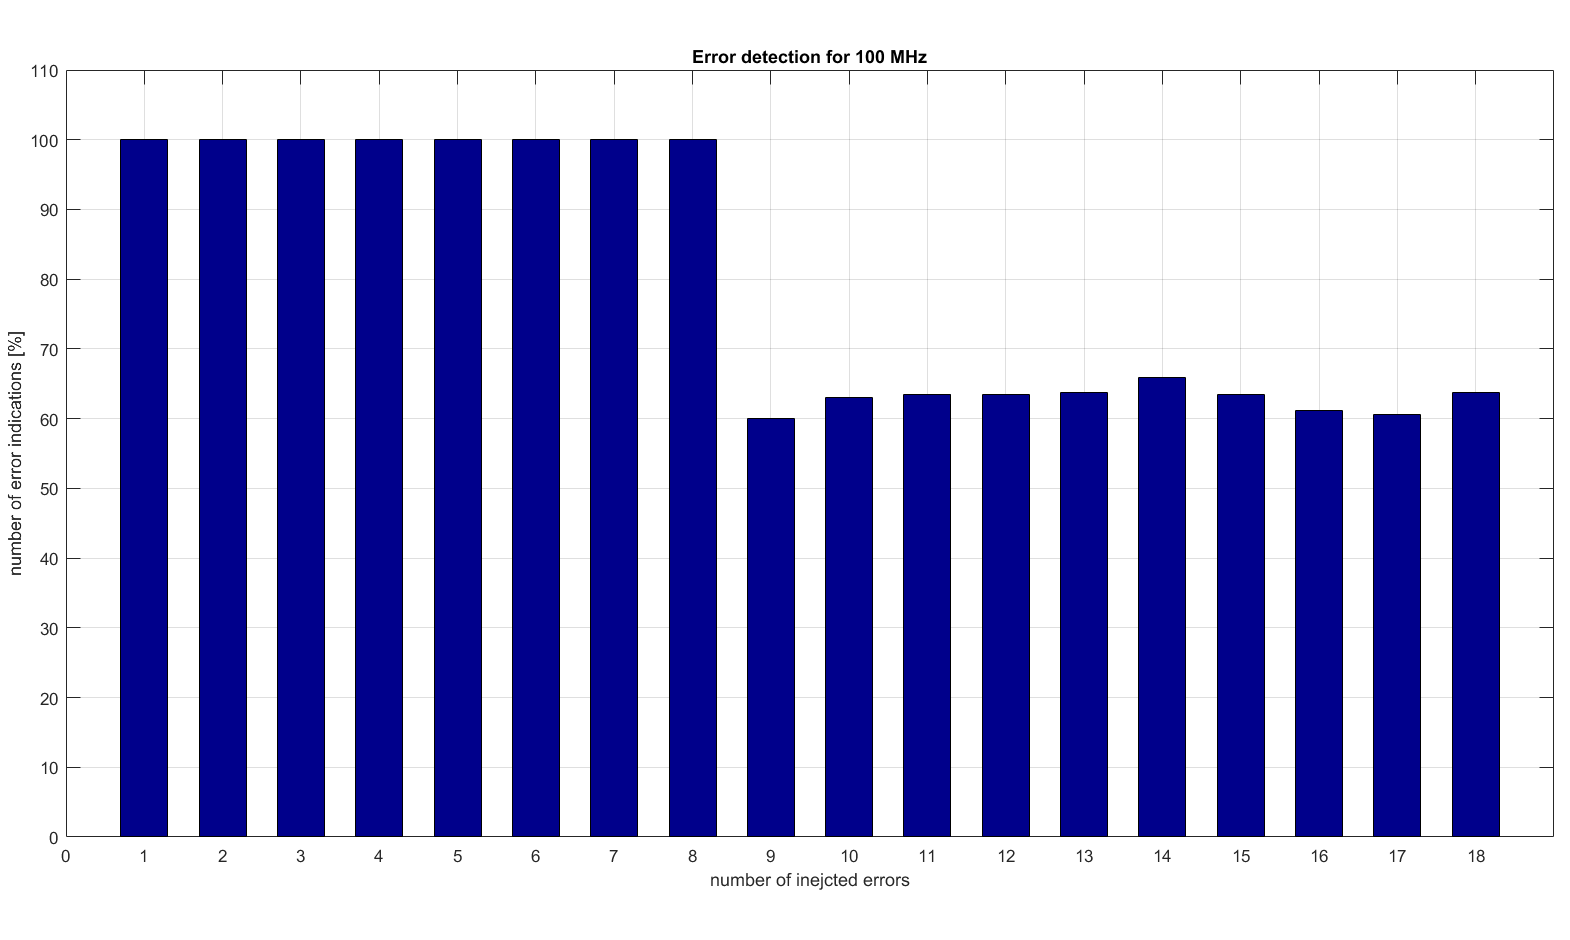
\includegraphics[width=\textwidth]{figures/max_detection_100.png}
\caption{The error detection limits of the decoder at 100 MHz}
\label{fig:dec_1}
\end{figure}

The decoder successfully detects and corrects all errors in those messages, where the number of errors does not exceed 8. It fails to correct any higher number of errors, giving a detection rate of about 63\%. A successful detection means that the code word was not simply accepted as fault-free and some sort of correction took place. The corrected bits don't necessarily correspond to the injected errors for error count above 8. The error vector simply transforms code words into invalid vectors laying somewhere within correction spheres of other code words. The miscorrection takes place, which transforms the vectors into invalid code words. The miscorrection is indistinguishable from normal correction and is not reported by the decoder, which is a disadvantage during the normal function. Since the BCH code is not a perfect code, the distances between neighboring code words are sometimes bigger than the minimal hamming distance of the code. The implication is that there is a possibility that a code word gets transformed by an error vector into an invalid vector laying outside of all error correcting spheres. Such situtation is not detected and the invalid vector gets accepted as a fault-free code word. The inability of error detection up to 16 bits shows that the decoder was implemented only for error correction purposes and does not present the full functionality of the underlaying code. The probability of detecting an error seams to be constant for any error number between 9 and 18 for normal function. It is a probability that any vector, with hamming distance from any code word equal to the number of injected faults, has simultaneously the hamming distance to any other code word smaller or equal 8, but not 0. 

Because the Test Engine allows tests with higher frequencies and the cut-off frequency of the decoder is known to be 220 MHz, the decoder was tested at 220 MHz for its maximal error detection. The result is shown in \autoref{fig:dec_2}. 

\begin{figure}[h]
\centering
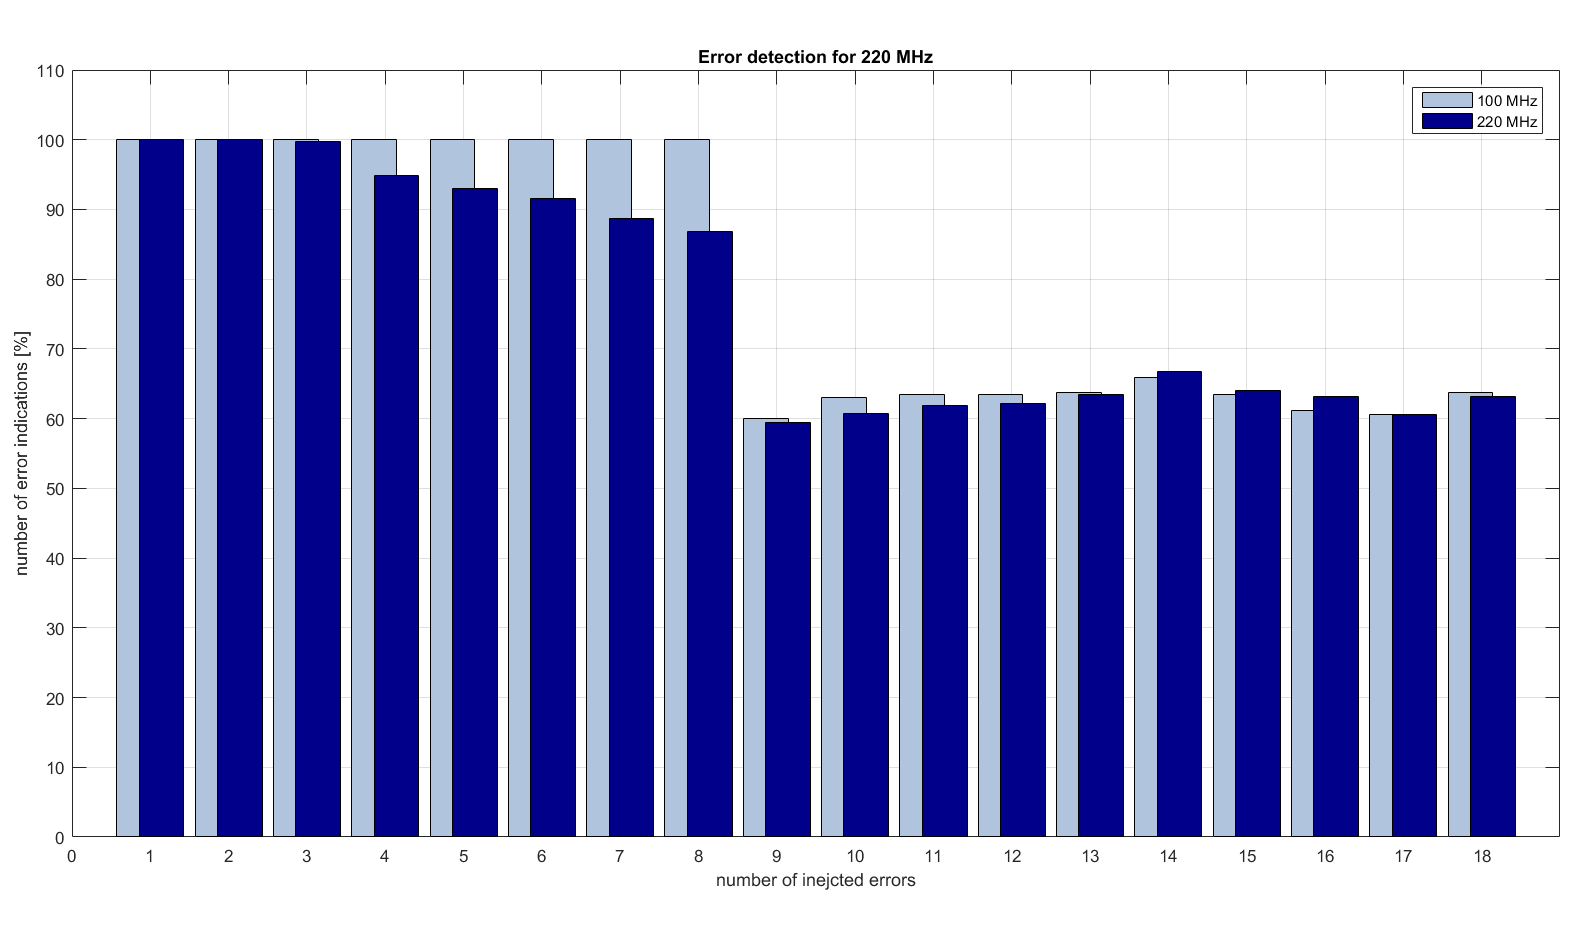
\includegraphics[width=\textwidth]{figures/max_detection_220.png}
\caption{The error detection limits of the decoder at 220 MHz}
\label{fig:dec_2}
\end{figure}

Another test was conducted at even higher frequency, to show a further decline in error detecting capabilities. The result of the test at 230 MHz is shown in \autoref{fig:dec_3}

\begin{figure}[h]
\centering
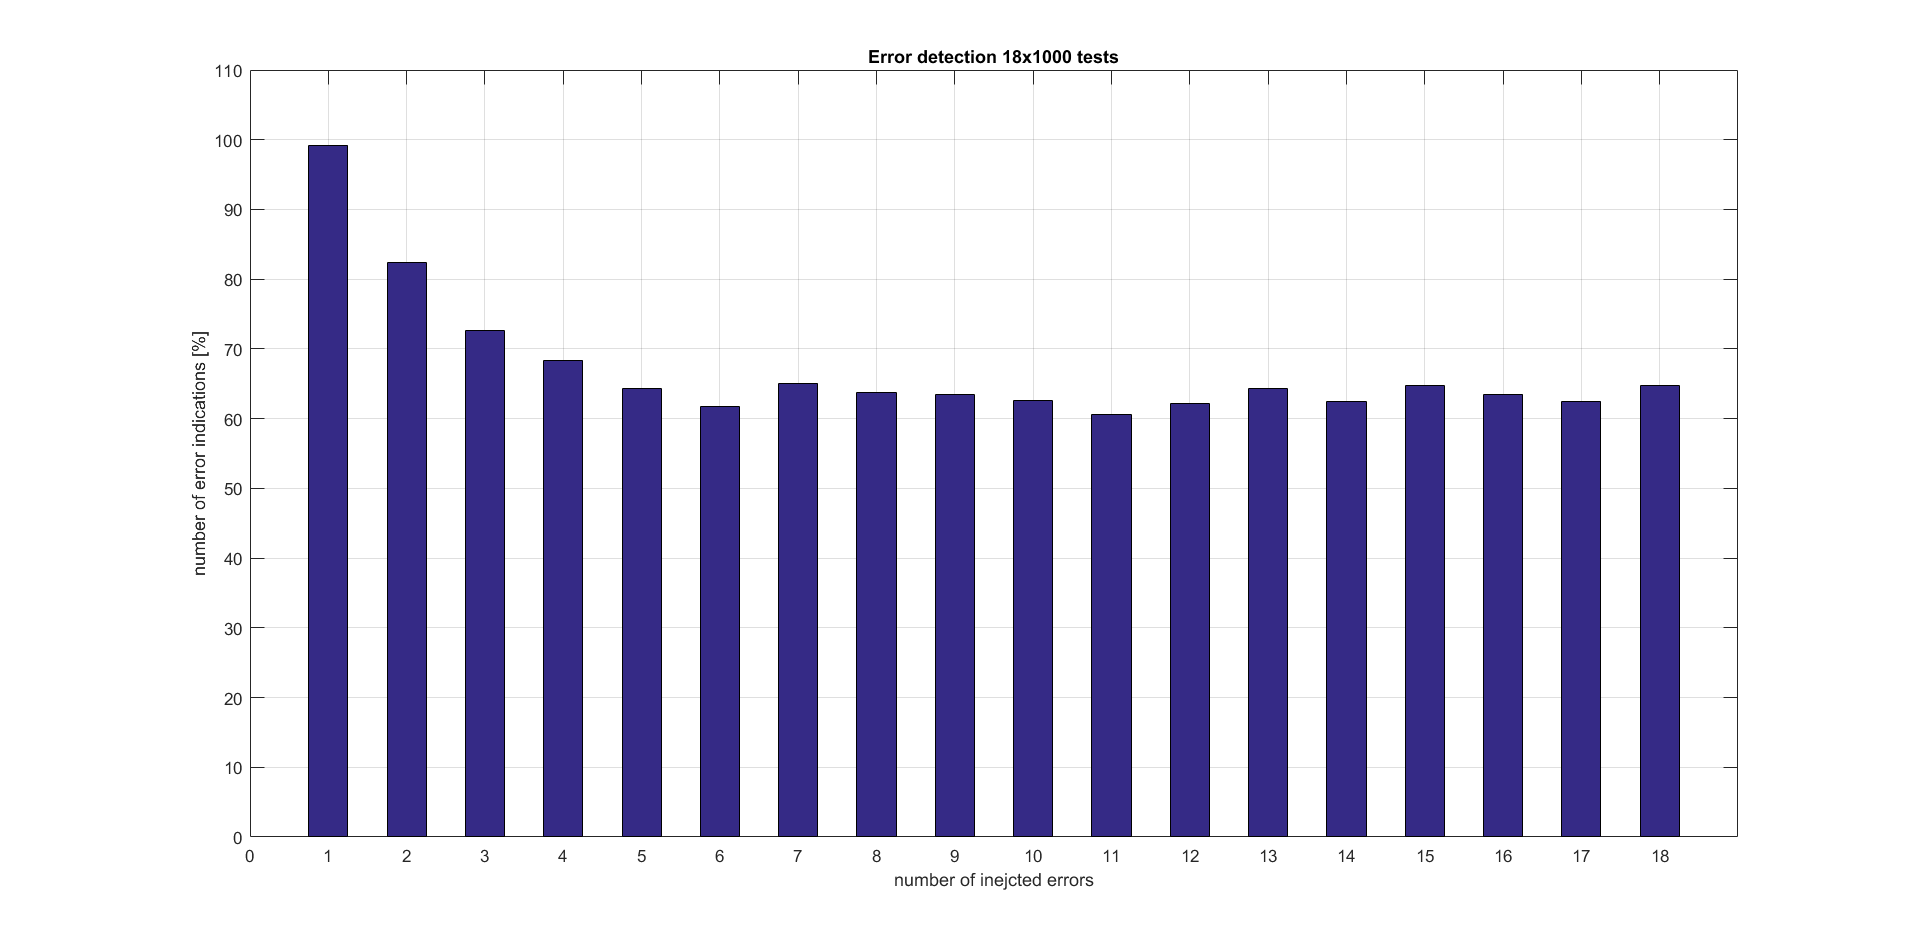
\includegraphics[width=\textwidth]{figures/max_detection_230.png}
\caption{The error detection limits of the decoder at 230 MHz}
\label{fig:dec_3}
\end{figure}

The error detection capability of the decoder was diminished by delay faults happening at the cut-off frequency and above. It fails to reliably detect any number of errors at 230 MHz and shows a significant decline of error detection by 220 MHz.

The error correction is also dependent on frequency and gets diminished at the cut-off frequency. The result of this degradation is visible in \autoref{fig:dec_4}.

\begin{figure}[h]
\centering
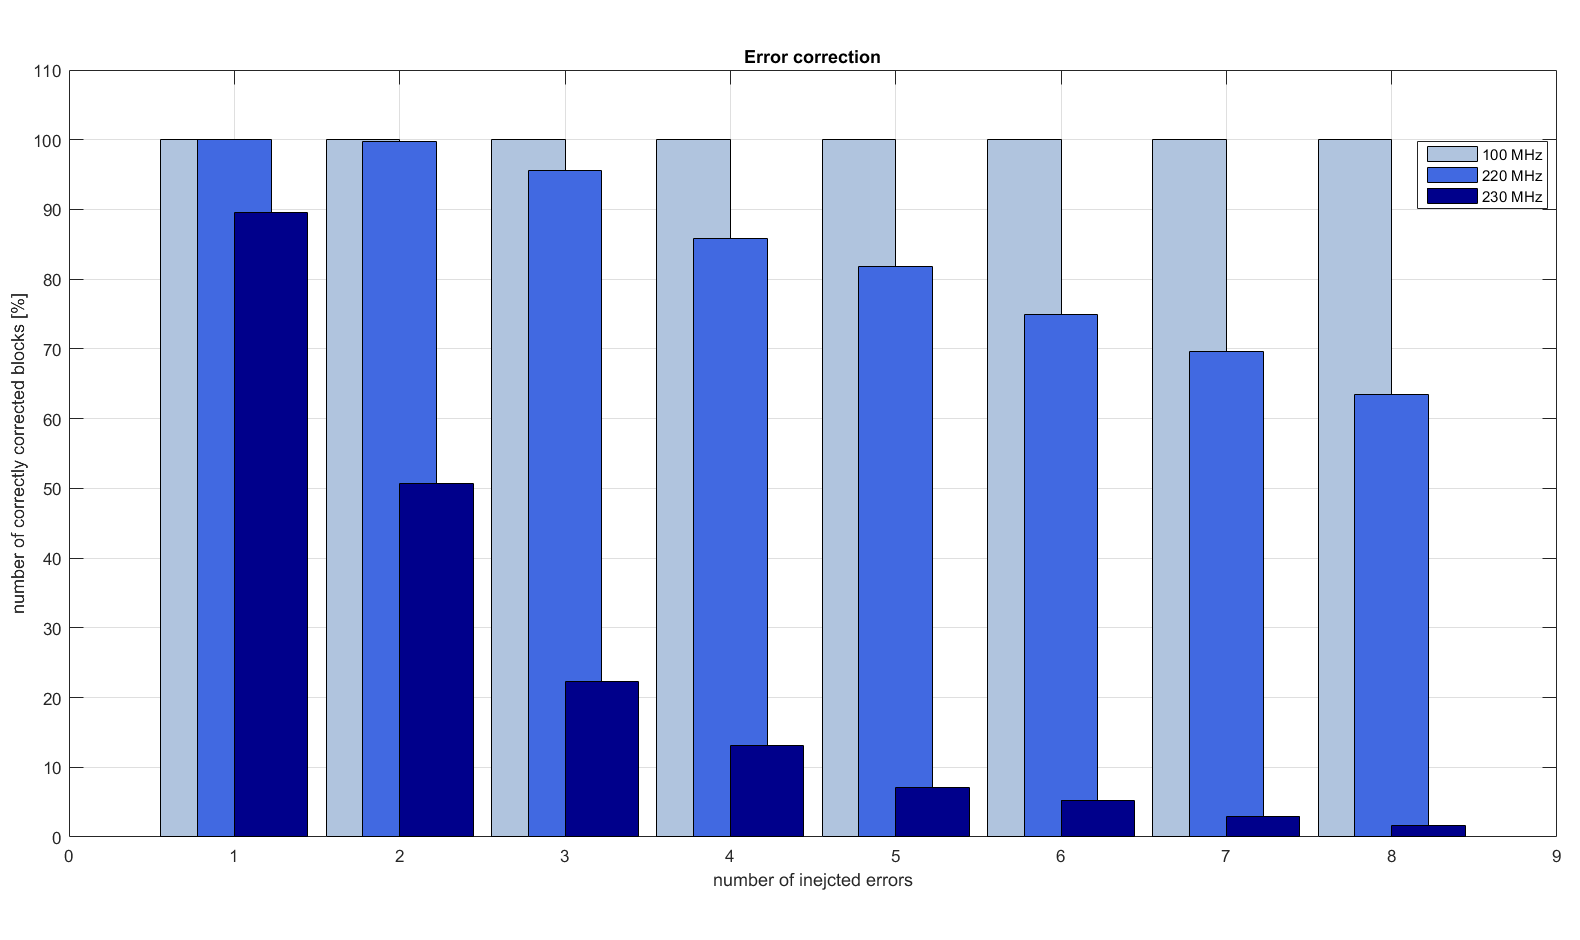
\includegraphics[width=\textwidth]{figures/max_correction.png}
\caption{The error correction limits of the decoder at different frequencies}
\label{fig:dec_4}
\end{figure}

\section{Systematic Test}

The diagnostic test is limited by the error detection capability of the decoder. The more errors a decoder can detect, the better chance of reliable test result. In systems with SEC-DED codes, like those implementing extended Hamming-code or Hsiao-code, the common weak point is erroneous error correction in case of triple bit errors and multiple bit errors \cite{art:Dicorato}. This weak point does not influence the Functional Short Test, since only the error detection counts. The exact error positions are not mandatory in case of a simple fail-pass test on module level. In case of multiple error detecting codes, like BCH code, the big latencies are not an issue during the test procedure, which makes them perfect candidates for the task of response analyzers.

Another limitation to the diagnostic test solution is the coverage of only those modules, which lay between encoder and decoder. The source encoding and cryptographic encryption are only two examples of modules that may reside outside of the test subsystem, not covered by the diagnostic test. For those modules, well established digital test methods need to be applied. The same restriction applies to the decoder architecture itself. It has been admittedly reported that some decoder architectures, like Hsiao-code decoder are capable of correcting (masking) some of its own hardware faults happening in the embedded encoder structure, under condition that they don't overlap with the transmission errors \cite{art:Dicorato}, but this feature does not cover the entire decoder structure and lowers the error coverage of the decoder. In the BCH decoder some delay faults caused only errors in parity bits, leaving the user bits intact. But in none of the cases does the diagnostic test cover the decoder internal faults. Therefore the decoder dependability needs to be taken care of separately. The diagnostic test can help in finding encoder or decoder faulty, since the last shortcut tests only those two modules. In case of failed test, as in all other cases, the repair of one unit is conducted and the test is repeated. The simpler solution is a BIST before the test procedure, with a self-repair possibility.

After making sure that the decoder is fault-free or got repaired using spare units, a systematic test can start. The first step is an exclusion of the communication channel. This can be achieved by local feedback. A direct connection between the receivers RF output and transmitters RF input through an attenuator. This is the first short-cut in the Functional Short System and is controlled by a MAC layer supervisor. The control during implementation is done externally by the user, based on the test results. The supervisor decides which shortcut should be taken and which test should be conducted. Before the functional test is started, it is good to run a BIST of any group capable of running such a test. The most important parts are those, which lay out of the main communication path. Those parts will not be tested during the functional test and should be tested in advance. These are for example LFSRs, which may be "rotated" and compared with known sequence to detect permanent faults. The same applies for modules outside of the test loop, like processors, which can be tested by creating an NMR system, running software test routines on all cores and comparing the results. In the ParSec system, special care needs to be given to the PHY unit, which is not accessible for internal test and can be tested only functionally. For any repair operation, if none is provided by the manufacturer, the duplication of the module is required. 

The test patterns are normal data frames, just used during the "fake" start-up. An off-line test before real start-up may uncover any permanent faults that may have prevented synchronization. Data packets should carry additional information about the number of detected errors. This information is crucial for controlling the test procedure. If the first functional test, consisting of many vectors, fails, a special counter connected to the $ISERR$ output of the decoder will indicate the number of detected errors. The information can also be coded, to contain the information about the error positions. Every decoder can output such data. If for example, errors were discovered in many vectors, exactly in the positions of parity bits, then with high probability the failing unit is the encoder. The information about error location can be valuable and used for optimizing the test flow.

The diagnostic functional test is used only for error detection. The repair of permanent faults require further redundancy, like spare units, leading to duplication of the hardware or parts of it. In case of patent protected circuitry, with no additional DfT extensions, a full duplication of hardware seems to be the only way to ensure repair possibility. Thanks to the diagnostic test, there is no need for tripling the hardware to create a TMR system.

When the first functional tests fail, the cause of the failure is definitely a hardware fault of one of the modules laying before the decoder. To locate the fault or faults, further narrowing of the test loop is necessary. If the test is run systematically and every short is taken one after another, the moment when the indication of detected errors disappears, will be the moment of isolating two suspected modules. Those two parts reside between the last taken shortcut and the one before the last. The fault may originate from the receiver or from the transmitter part. Without further testing, a self-repair of one of the modules has to be conducted, to see if the error disappeared. The self-repair procedure is only possible by reconfiguration and use of a spare unit, to substitute the failed one. If the error didn't disappear, the self repair needs to be reverted and the other module repaired. The information about the error position can be used to choose how the self-repair should be conducted. In case of a Hsiao-Code encoder, this information can unambiguously point to the faulty unit, responsible for the error, making the BIST of the encoder redundant.

While SEC-DED decoders repair also some of the encoder faults, in case of the BCH encoder, any fault in the LFSR causes a multiple bit error beyond any error detection capabilities. The tested decoder can however detect over 60\% of erroneous blocks, which may be enough to run the functional test. As alternative, a BIST for the encoder is suggested, at best to run before the functional test. An example of BIST for LFSRs is given in \cite{art:Gleichner}. The LFSR are operated as shift registers, with their feedback disabled. After the seeding pattern is shifted in, the feedback gets enabled and the LFSR runs for several clock cycles, until it contains the seeding pattern again. This state is compared with the initial one. In case of any difference, the permanent fault gets detected. The LFSRs are very regular units, therefore a repair using spare parts is easy to implement.

Another small drawback of the shortcut system is the overhead in multiplexing. The additional multiplexers, laying on transmission path, lead to signal deterioration, which is especially important in the analog part. The multiplexers need to be adjusted, so that their response does not disturb "normal" functionality of the system. In digital logic, the additional multiplexers create additional delay, although the switching happens off-line, so it should not influence the "normal" function.

\section{Summary}

In conclusion, the suggested solution is useful as diagnostic test in systems with no internal access to some modules laying between FEC encoder and decoder and allows the test of analog, mixed-signal and digital modules indifferently with just little hardware and software overhead. The test is limited by error detection capability of the decoder. The limitation is not different than the test result evaluation using signatures. The tests are false positive in case of error vectors changing one code word into another valid code word, just like conflicts happening in signature calculation. While there is no guarantee, some decoders can correctly qualify many vectors as faulty, even though their error count exceeds decoders detecting capabilities.

The results of tests conducted on encoder and decoder architectures, helped by the development process and were a valuable input in understanding the limitations of the tested designs. They also validated the proper functionality of the basic PENCA building blocks and showed, in case of decoder, where are the possible bottlenecks. Unfortunately, the test engine was not successful in testing the limits of the encoder architecture.

As a result of this thesis, a useful tool for design validation in "real" hardware was developed and may be used as an alternative to simulation, speeding up the development process and allowing quick evaluation of responses with any chosen program. The placement of the design is to be treated with much caution and understanding, to avoid misinterpretation of the test results.